
\section{Exercise 4}

\begin{quoting}
  Repeat Exercise (2e), but use a more advanced prediction model (your
  choice) to estimate the propensity score. Describe ($\sim$3
  sentences) any differences.
\end{quoting}

We performed a probit regression using Bayesian additive regression
trees \citep[BART;][]{chipman2010} with the \texttt{dbarts} package in
\textsf{R} to estimate the propensity score.  We estimated the
treatment effect with weighted least squares using these weights for
the linear model in Eq.~\eqref{eq:lin-mod}, similarly to Problem 3(e).
\begin{itemize}
\item 2002: -0.6651 (SE = 0.0434)
\item 2014: -0.8018 (SE = 0.0410) 
\end{itemize}

Note that the estimated treatment effect is slightly lower for year
2002, and much lower for year 2014.  These differences arise entirely
from the discrepancy in the estimated propensity scores between
logistic regression and from BART.

Figure~\ref{fig:prop-comp} compares the propensity scores estimated
from logistic regression (as used in all of Problem 2) to those
estimated from BART. For the both years, BART tends to give a lower
propensity score for control units ($Z=0$), and a higher propensity
score for treatment units ($Z=1$).  This pattern is especially notable
for year 2014.  This suggests that BART might be ``overfitting'' the
estimated propensity score model.

\begin{figure}[ht]
  \centering
  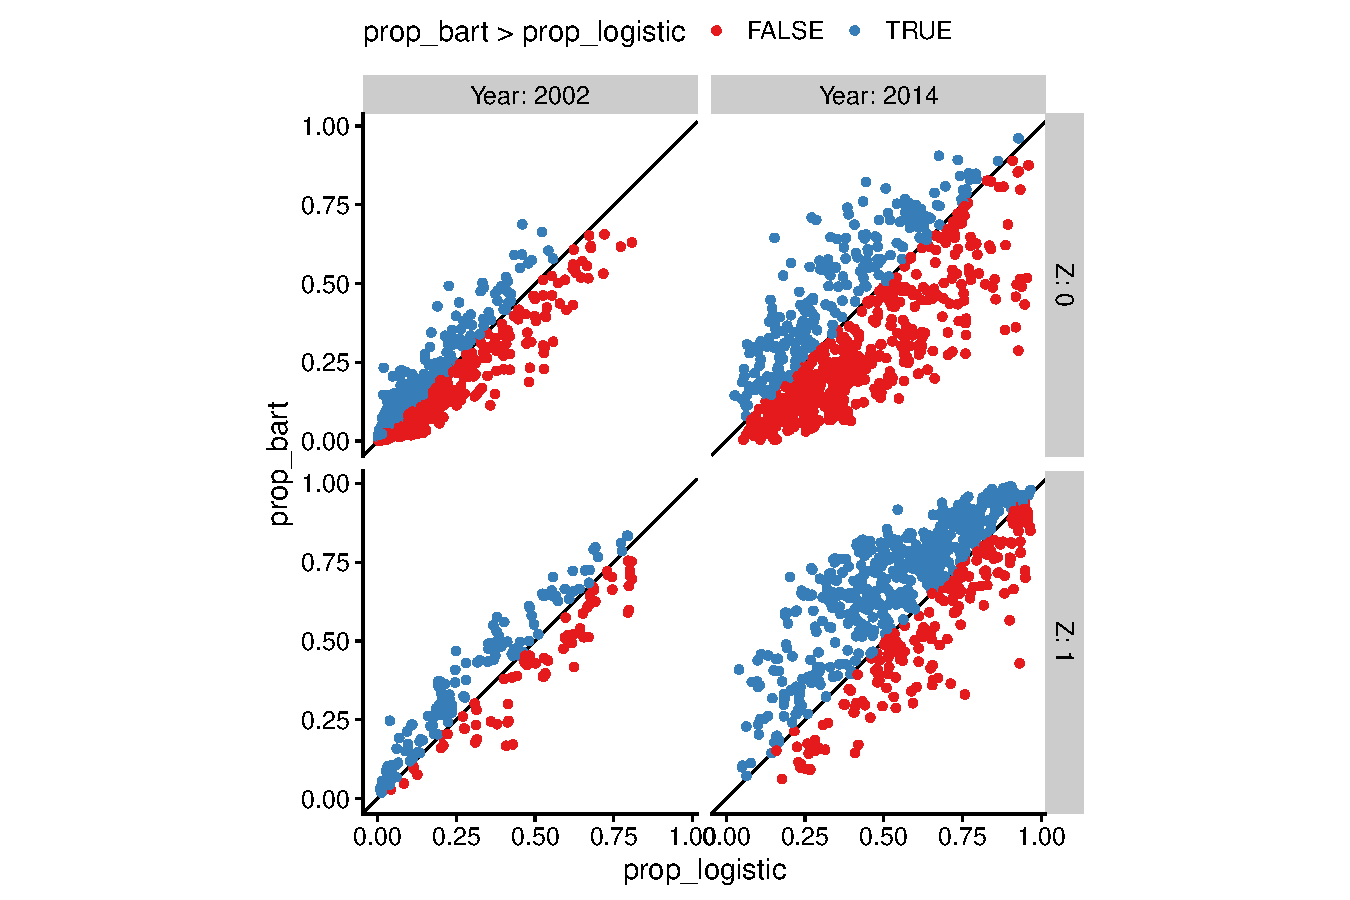
\includegraphics[width=0.8\textwidth]{figures/prop-comp}
  \caption{\label{fig:prop-comp} Comparison of estimated propensity scores from logistic regression and BART. }
\end{figure}


%%% Local Variables:
%%% mode: latex
%%% TeX-master: "../main"
%%% End:
